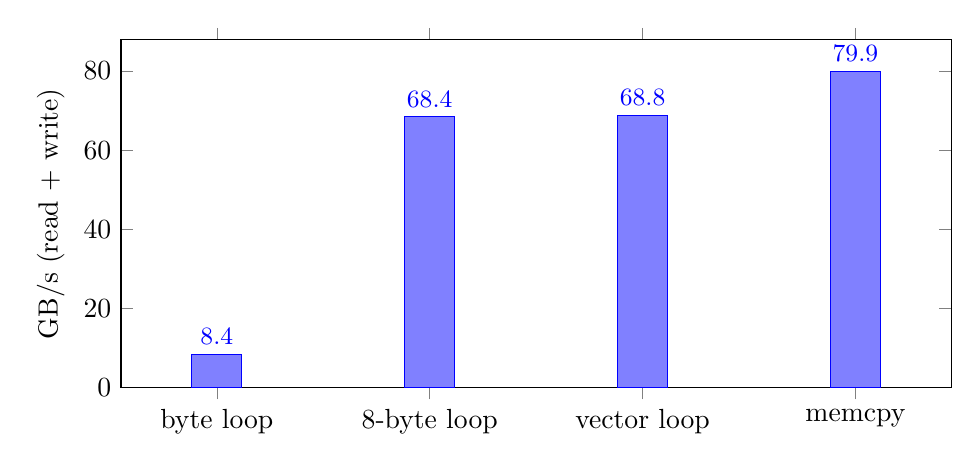
\begin{tikzpicture}
\begin{axis}[ybar, width=\textwidth, height=6cm, bar width=18pt, ymin=0, ylabel={GB/s (read + write)}, symbolic x coords={byte loop,8-byte loop,vector loop,memcpy}, xtick=data, nodes near coords, nodes near coords style={font=\small}, enlarge x limits=0.15]
\addplot+[fill=blue!50] coordinates {(byte loop,8.4) (8-byte loop,68.4) (vector loop,68.8) (memcpy,79.9)};
\end{axis}
\end{tikzpicture}